\documentclass{beamer}

\usepackage{comment}
\usepackage{color}
\usepackage{listings}
\usepackage{verbatim}
\usepackage{multicol}
\usepackage{booktabs}
\definecolor{green}{RGB}{0,128,0}

\newcommand\gehcomment[1]{{{\color{orange} #1}}}
\newcommand\add[1]{{{\color{blue} #1}}}
\newcommand\remove[1]{\sout{{\color{red} #1}}}
\newcommand\codecomment[1]{{{\color{green} #1}}}
\newcommand\redcomment[1]{{{\color{red} #1}}}
\newcommand\bluecomment[1]{{{\color{blue} #1}}}
\newcommand\greencomment[1]{{{\color{green} #1}}}
\newcommand\magentacomment[1]{{{\color{magenta} #1}}}

\begin{comment}
\tiny
\scriptsize
\footnotesize
\small
\normalsize
\large
\Large
\LARGE
\huge
\Huge
\end{comment}

\begin{document}
\title{Multiphase - Gas Injection}
\author{Emily Stein}
\date{\today}

%\frame{\titlepage}

%-----------------------------------------------------------------------------
\section{Description of Heater}

\subsection{Heater Conceptual Model}

\begin{frame}\frametitle{Description of Heater Scenario}
The ``Heater Scenario'' demonstrates how to set up a multiphase flow simulation using GENERAL MODE. It simulates a heat source (such as radioactive waste) in a partially saturated domain. Assumptions include:
\begin{itemize}
  \item Problem domain: $15 \times 1 \times 30$ m (x $\times$ y $\times$ z)
  \item Grid resolution: Varies in an unstructured grid
  \item Flow mode: General
  \item Heat Source: Rate scaled by cell volume
  \item Maximum time step size: changes with simulation time
  \item Total simulation time: 1000 d
\end{itemize}

\end{frame}

%-----------------------------------------------------------------------------
\frame{\frametitle{2D Heater Scenario Schematic}
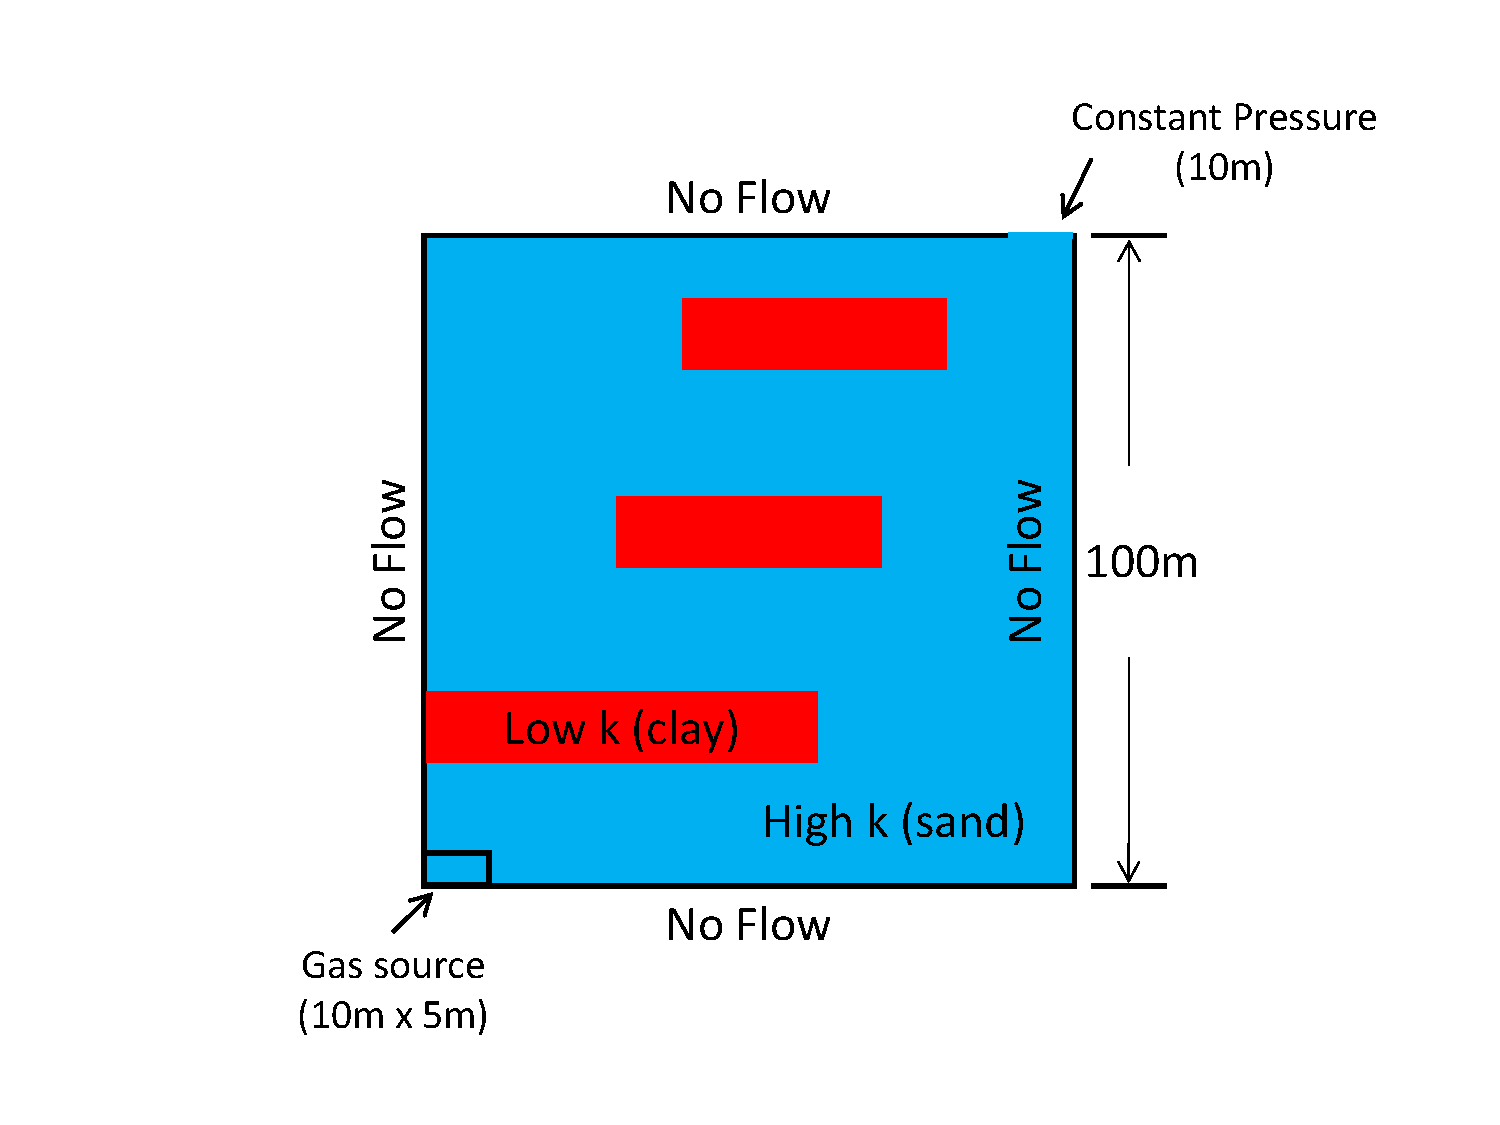
\includegraphics[width=\linewidth]{./gas_injection_bc}
}

%-----------------------------------------------------------------------------
\frame{\frametitle{2D Heater Initial Conditions}
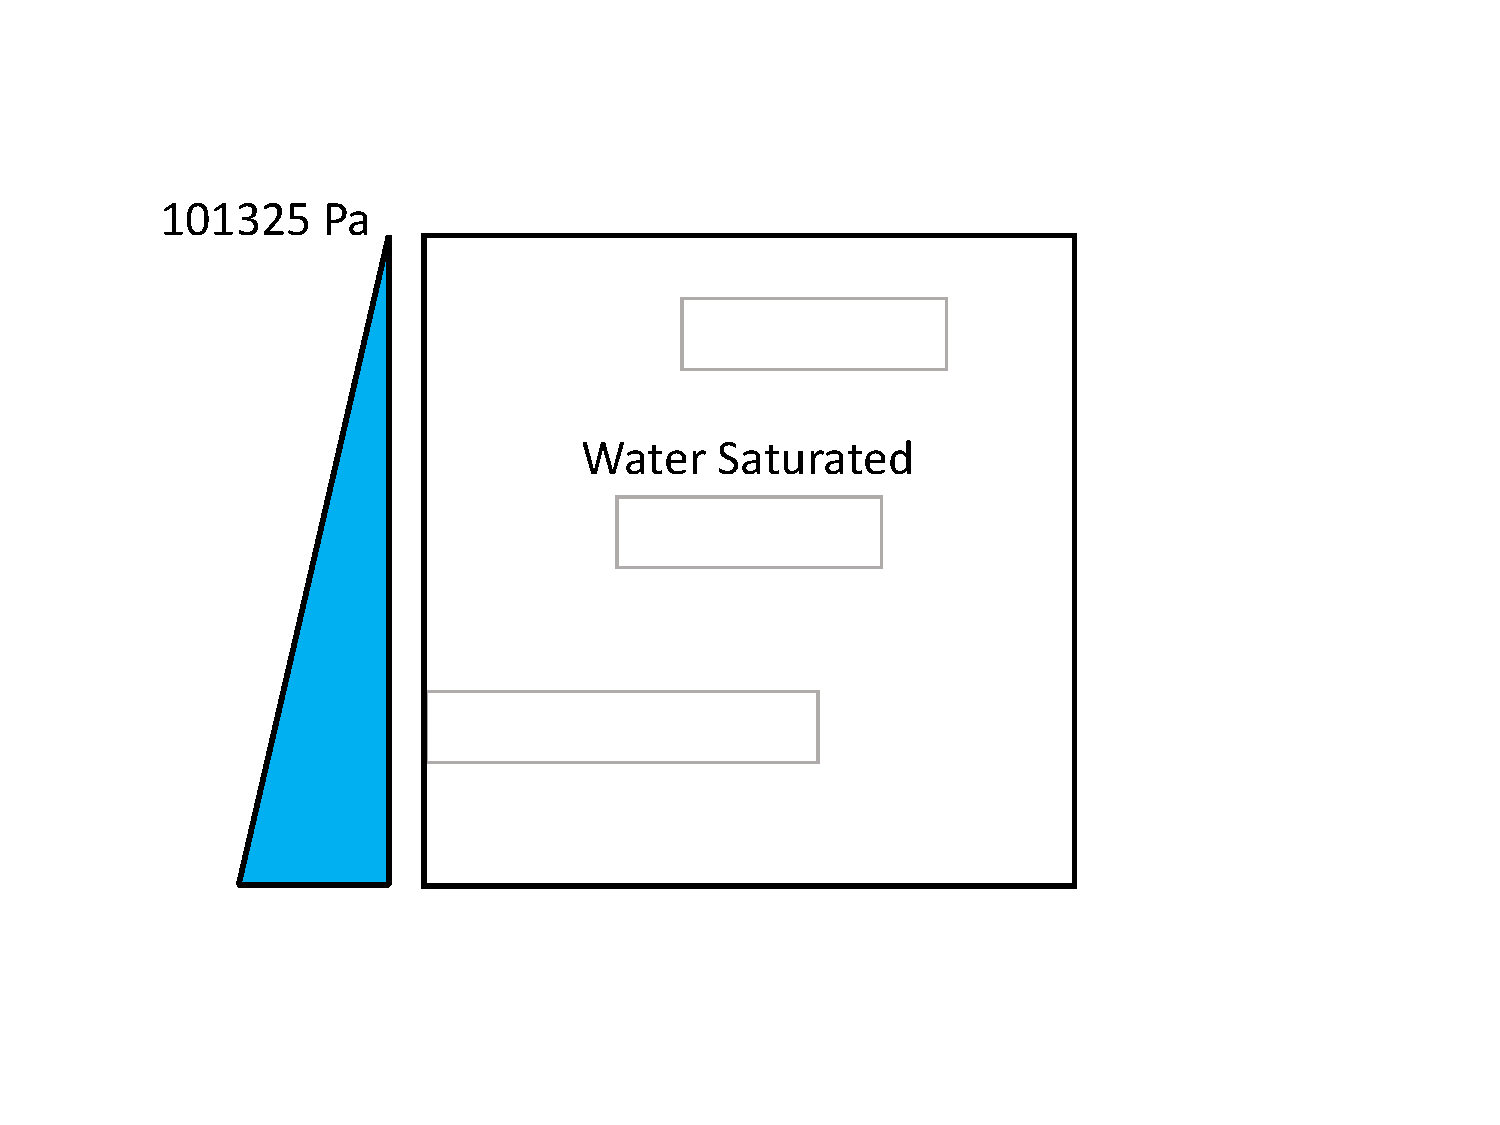
\includegraphics[width=\linewidth]{./gas_injection_ic}
}

%-----------------------------------------------------------------------------
\section{Description of Input Deck}

%-----------------------------------------------------------------------------
\subsection{SIMULATION}

\begin{frame}[fragile]\frametitle{SIMULATION}

\begin{itemize}
  \item Multiphase flow (General mode)
  \item with options
\end{itemize}

\begin{semiverbatim}\small
SIMULATION
  SIMULATION_TYPE SUBSURFACE
  PROCESS_MODELS
    SUBSURFACE_FLOW flow
      MODE GENERAL ! two-phase flow and energy
      OPTIONS
        ANALYTICAL_DERIVATIVES
      /   
    /   
  /
END

SUBSURFACE
...
END_SUBSURFACE
\end{semiverbatim}

\end{frame}

%-----------------------------------------------------------------------------
\subsection{GRID}

\begin{frame}[fragile]\frametitle{GRID}

\begin{itemize}
  \item Problem domain: $15 \times 1 \times 30$ m (x $\times$ y $\times$ z)
  \item Grid resolution: Varies in unstructured grid
\end{itemize}

\begin{semiverbatim}
GRID
  TYPE UNSTRUCTURED ./heater.h5
END
\end{semiverbatim}

\end{frame}

%-----------------------------------------------------------------------------
\subsection{FLUID\_PROPERTY}

\begin{frame}[fragile]\frametitle{FLUID\_PROPERTY}
\begin{itemize}
  \item Diffusion of dissolved gas in water
  \item Diffusion of water vapor in gas
\end{itemize}

\begin{semiverbatim}

FLUID_PROPERTY
  PHASE LIQUID \bluecomment{! for diffusion of dissolved gas}
  DIFFUSION_COEFFICIENT 1.d-9
END

FLUID_PROPERTY
  PHASE GAS \bluecomment{! for diffusion of water vapor}
  DIFFUSION_COEFFICIENT 2.1d-5
END
\end{semiverbatim}

\end{frame}

%-----------------------------------------------------------------------------
\subsection{OUTPUT}

\begin{frame}[fragile]\frametitle{OUTPUT}
\begin{itemize}
  \item Print a snapshot of entire solution periodically
  \item Print the solution at observation points every time step
  \item Print mass balance file every time step
  \item Choose output variables
\end{itemize}

\end{frame}

\begin{frame}[fragile]\frametitle{OUTPUT}

\begin{semiverbatim}\small
OUTPUT
  SNAPSHOT_FILE
    FORMAT HDF5
    PERIODIC TIME .1 d between 0. d and .1 d \bluecomment{! print every 0.1 day}
    PERIODIC TIME 1. d between 0. d and 10. d  \bluecomment{! then every 1. day}
    PERIODIC TIME 10. d between 0. d and 100. d  \bluecomment{! etc.}
    PERIODIC TIME 100. d between 0. d and 1000. d
  /
  OBSERVATION_FILE
    PERIODIC TIMESTEP 1 \bluecomment{! print every time step}
  /
  MASS_BALANCE_FILE
    PERIODIC TIMESTEP 1 \bluecomment{! print every time step}
  /
  VELOCITY_AT_CENTER \bluecomment{! of cell}
  VARIABLES
    TEMPERATURE
    LIQUID_SATURATION
    GAS_SATURATION \bluecomment{! see input deck for more}
  /
END
\end{semiverbatim}

\end{frame}

%-----------------------------------------------------------------------------
\subsection{TIME}

\begin{frame}[fragile]\frametitle{TIME}
\begin{itemize}
  \item Final simulation time = 100 y
  \item Maximum time step size = 5 y
\end{itemize}

\begin{semiverbatim}

TIME
  FINAL_TIME 1000.d0 d \bluecomment{! end of simulation}
  MAXIMUM_TIMESTEP_SIZE .1 d at 0. d \bluecomment{! start small}
  MAXIMUM_TIMESTEP_SIZE 1. d at 1. d \bluecomment{! allow larger}
  MAXIMUM_TIMESTEP_SIZE 10. d at 10. d \bluecomment{! at late times}
  MAXIMUM_TIMESTEP_SIZE 100. d at 100. d
END
\end{semiverbatim}

\end{frame}

%-----------------------------------------------------------------------------
\subsection{MATERIAL\_PROPERTY}

\begin{frame}[fragile]\frametitle{MATERIAL\_PROPERTY}
\begin{itemize}
  \item Energy equations require:
  \begin{itemize}
    \item mineral density
    \item thermal conductivity
    \item mineral heat capacity
  \end{itemize}
\end{itemize}

\begin{semiverbatim}\small
MATERIAL_PROPERTY shale
  ID 4
  CHARACTERISTIC_CURVES default
  POROSITY 0.20
  TORTUOSITY 0.11
  ROCK_DENSITY 2700. \bluecomment{! density of the solid phase}
  THERMAL_CONDUCTIVITY_DRY 1.0d0 \bluecomment{! dry bulk medium}
  THERMAL_CONDUCTIVITY_WET 1.7d0 \bluecomment{! wet bulk medium}
  HEAT_CAPACITY 830. \bluecomment{! heat capacity of the solid phase}
  PERMEABILITY
    PERM_ISO 1.d-19
  /
END
\end{semiverbatim}
\end{frame}

\begin{frame}[fragile]\frametitle{MATERIAL\_PROPERTY}
\begin{semiverbatim}
MATERIAL_PROPERTY drz
  ID 3
  CHARACTERISTIC_CURVES drz
  POROSITY 0.20
  TORTUOSITY 0.11
  ROCK_DENSITY 2700. \bluecomment{! density of the solid phase}
  THERMAL_CONDUCTIVITY_DRY 1.0d0 \bluecomment{! dry bulk medium}
  THERMAL_CONDUCTIVITY_WET 1.7d0 \bluecomment{! wet bulk medium}
  HEAT_CAPACITY 830. \bluecomment{! heat capacity of the solid phase}
  PERMEABILITY
    PERM_ISO 1.d-18
  /
END
\end{semiverbatim}
\end{frame}

\begin{frame}[fragile]\frametitle{MATERIAL\_PROPERTY}
\begin{semiverbatim}
MATERIAL_PROPERTY bentonite
  ID 2
  CHARACTERISTIC_CURVES bentonite
  POROSITY 0.35
  TORTUOSITY 0.23
  ROCK_DENSITY 2700. \bluecomment{! density of the solid phase}
  THERMAL_CONDUCTIVITY_DRY 0.6d0 \bluecomment{! dry bulk medium}
  THERMAL_CONDUCTIVITY_WET 1.2d0 \bluecomment{! wet bulk medium}
  HEAT_CAPACITY 830. \bluecomment{! heat capacity of the solid phase}
  PERMEABILITY
    PERM_ISO 1.d-20
  /
END
\end{semiverbatim}
\end{frame}

\begin{frame}[fragile]\frametitle{MATERIAL\_PROPERTY}
\begin{semiverbatim}
MATERIAL_PROPERTY heater
  ID 1
  CHARACTERISTIC_CURVES default
  POROSITY 0.01 ! a small value
  TORTUOSITY 1.0
  ROCK_DENSITY 5000. \bluecomment{! density of the solid phase}
  THERMAL_CONDUCTIVITY_DRY 16.7d0 \bluecomment{! dry bulk medium}
  THERMAL_CONDUCTIVITY_WET 16.7d0 \bluecomment{! wet bulk medium}
  HEAT_CAPACITY 466. \bluecomment{! heat capacity of the solid phase}
  PERMEABILITY
    PERM_ISO 1.d-23 ! a small value
  /
END
\end{semiverbatim}
\end{frame}
%-----------------------------------------------------------------------------
\subsection{CHARACTERISTIC\_CURVES}

\begin{frame}[fragile,containsverbatim]\frametitle{CHARACTERISTIC\_CURVES}
\begin{itemize}
  \item Van Genuchten/Mualem
\end{itemize}
\begin{semiverbatim}\small
CHARACTERISTIC_CURVES default
  SATURATION_FUNCTION VAN_GENUCHTEN
    ALPHA 1.d-4
    M 0.5
    LIQUID_RESIDUAL_SATURATION 0.1d0
  /
  PERMEABILITY_FUNCTION MUALEM_VG_LIQ
    PHASE LIQUID
    M 0.5
    LIQUID_RESIDUAL_SATURATION 0.1d0
  /
  PERMEABILITY_FUNCTION MUALEM_VG_GAS
    PHASE GAS
    M 0.5
    LIQUID_RESIDUAL_SATURATION 0.1d0
    GAS_RESIDUAL_SATURATION 0.1d0
  /
END
\end{semiverbatim}
\end{frame}

\begin{frame}[fragile,containsverbatim]\frametitle{CHARACTERISTIC\_CURVES}
\begin{itemize}
  \item Van Genuchten/Mualem
\end{itemize}
\begin{semiverbatim}\small
CHARACTERISTIC_CURVES shale
  SATURATION_FUNCTION VAN_GENUCHTEN
    ALPHA 7.d-7
    M 0.333
    LIQUID_RESIDUAL_SATURATION 0.1d0
  /
  PERMEABILITY_FUNCTION MUALEM_VG_LIQ
    PHASE LIQUID
    M 0.333
    LIQUID_RESIDUAL_SATURATION 0.1d0
  /
  PERMEABILITY_FUNCTION MUALEM_VG_GAS
    PHASE GAS
    M 0.333
    LIQUID_RESIDUAL_SATURATION 0.1d0
    GAS_RESIDUAL_SATURATION 0.1d0
  /
END
\end{semiverbatim}
\end{frame}

\begin{frame}[fragile,containsverbatim]\frametitle{CHARACTERISTIC\_CURVES}
\begin{itemize}
  \item Van Genuchten/Mualem
\end{itemize}
\begin{semiverbatim}\small
CHARACTERISTIC_CURVES bentonite
  SATURATION_FUNCTION VAN_GENUCHTEN
    ALPHA 6.d-8
    M 0.375
    LIQUID_RESIDUAL_SATURATION 0.1d0
  /
  PERMEABILITY_FUNCTION MUALEM_VG_LIQ
    PHASE LIQUID
    M 0.375
    LIQUID_RESIDUAL_SATURATION 0.1d0
  /
  PERMEABILITY_FUNCTION MUALEM_VG_GAS
    PHASE GAS
    M 0.375
    LIQUID_RESIDUAL_SATURATION 0.1d0
    GAS_RESIDUAL_SATURATION 0.1d0
  /
END
\end{semiverbatim}
\end{frame}
%-----------------------------------------------------------------------------
\subsection{REGION}

\begin{frame}[fragile]\frametitle{REGION}
\begin{itemize}
  \item{Entire domain}
  \item{Regions for initial conditions}
  \item{Region for boundary condition}
\end{itemize}

\begin{semiverbatim}\small
REGION all
  COORDINATES
    -1.d20 -1.d20 -1.d20 \bluecomment{! very large volume}
     1.d20  1.d20  1.d20 \bluecomment{! nothing will be left out}
  /
END

REGION Region1 \bluecomment{! heater}
  FILE ./heater_usg.h5
END

REGION Region2 \bluecomment{! bentonite}
  FILE ./heater_usg.h5
END

REGION outer_face \bluecomment{! for b.c.}
  FILE ./heater_usg.h5
END
\end{semiverbatim}
\end{frame}
%-----------------------------------------------------------------------------
\subsection{OBSERVATION}

\begin{frame}[fragile]\frametitle{OBSERVATION}
\begin{itemize}
  \item{Define two more regions for output}
\end{itemize}

\begin{semiverbatim}\small
REGION bentonite_obs
  COORDINATE 1.3d0 0.5d0 0.d0
/
REGION drz_obs
  COORDINATE 2.6d0 0.5d0 0.d0
/

OBSERVATION
  REGION bentonite_obs
/
OBSERVATION
  REGION drz_obs
/
\end{semiverbatim}
\end{frame}

%-----------------------------------------------------------------------------
\subsection{FLOW\_CONDITION}

\begin{frame}[fragile]\frametitle{FLOW\_CONDITION}
\begin{itemize}
  \item{Single phase liquid, hydrostatic}
\end{itemize}

\begin{semiverbatim}
FLOW_CONDITION initial_shale \bluecomment{! single phase liquid}
  TYPE
    LIQUID_PRESSURE HYDROSTATIC
    MOLE_FRACTION DIRICHLET
    TEMPERATURE DIRICHLET
  /
  DATUM 0.d0 0.d0 0.d0 \bluecomment{! center of drift}
  LIQUID_PRESSURE 5.d6 \bluecomment{! Pa}
  MOLE_FRACTION 1.d-8 \bluecomment{! dissolved gas}
  TEMPERATURE 25.d0 \bluecomment{! degrees C}
END
\end{semiverbatim}
\end{frame}

\begin{frame}[fragile]\frametitle{FLOW\_CONDITION}
\begin{itemize}
  \item{Two-phase}
\end{itemize}

\begin{semiverbatim}
FLOW_CONDITION initial_bentonite \bluecomment{! two-phase}
  TYPE
    GAS_PRESSURE DIRICHLET
    GAS_SATURATION DIRICHLET
    TEMPERATURE DIRICHLET
  /
  GAS_PRESSURE 101325.d0 \bluecomment{! Pa}
  GAS_SATURATION 0.8d0
  TEMPERATURE 25.d0 \bluecomment{! degrees C}
END
\end{semiverbatim}
\end{frame}

\begin{frame}[fragile]\frametitle{FLOW\_CONDITION}
\begin{itemize}
  \item{Source term}
\end{itemize}

\begin{semiverbatim}
FLOW_CONDITION heater
  TYPE
    RATE SCALED_MASS_RATE VOLUME \bluecomment{! volume averaged}
  /
  SYNC_TIMESTEP_WITH_UPDATE
  RATE LIST
    TIME_UNITS d
    DATA_UNITS kg/s kg/s W
    \bluecomment{! time liquid gas energy}
    0.d0 0.d0 0.d0 0.d0
    .1d0 0.d0 0.d0 100.d0
    365.d0 0.d0 0.d0 0.d0
  /
END
\end{semiverbatim}
\end{frame}

%-----------------------------------------------------------------------------
\subsection{Couplers}

\begin{frame}[fragile]\frametitle{Couplers}

\begin{itemize}
  \item Initial condition with region
  \item Boundary condition with region
  \item Source (or sink) with region
\end{itemize}

\begin{semiverbatim}\small
\bluecomment{! initial condition}
INITIAL_CONDITION shale \bluecomment{! optional name}
  FLOW_CONDITION initial_shale
  REGION all
END

INITIAL_CONDITION heater \bluecomment{! optional name}
  FLOW_CONDITION initial_bentonite
  REGION Region1
END

INITIAL_CONDITION bentonite \bluecomment{! optional name}
  FLOW_CONDITION initial_bentonite
  REGION Region2
END
\end{semiverbatim}
\end{frame}

\begin{frame}
\begin{semiverbatim}
\bluecomment{! boundary condition}
BOUNDARY_CONDITION open \bluecomment{! optional name}
  FLOW_CONDITION initial_shale
  REGION outer_face
END
\bluecomment{! source_sink }
SOURCE_SINK heat \bluecomment{! optional name}
  FLOW_CONDITION heatsource
  REGION Region1
END
\end{semiverbatim}
\end{frame}

\begin{frame}[fragile]\frametitle{Couplers}

\begin{itemize}
  \item{Material with region}
\end{itemize}

\begin{semiverbatim}
STRATA
  MATERIAL ./heater_usg.h5
END

END_SUBSURFACE \bluecomment{! That's all!}
\end{semiverbatim}
\end{frame}

%-----------------------------------------------------------------------------
\subsection{Command Line}
\begin{frame}[fragile]\frametitle{Command Line}
\begin{semiverbatim}
\$ pflotran -input_prefix heater
\end{semiverbatim}

\end{frame}

%-----------------------------------------------------------------------------
\end{document}
